\chapter{Extract Hashes}
Una parte fondamentale dei attacchi Brute-Force è il fatto di recuperare gli hash, in modo da poterli attaccare offline, andando a ridure cosi i tempi e le tracce che si possono lasciare.
Questi hash possono trovarsi in vari sistemi, diversi tra loro e ognuno si differenzia per il modo e per i strumenti con cui si possono recuperare.
\section{Windows}
In Windows gli hash inerenti alle password dei account, sono archiviati in un file di database nel controller di dominio (NTDS.DIT) con alcune informazioni aggiuntive come le appartenenze ai gruppi e gli utenti.

Il file NTDS.DIT è costantemente utilizzato dal sistema operativo e quindi non può essere copiato direttamente in un'altra posizione per l'estrazione delle informazioni.
\begin{lstlisting}[ caption={NTDS.DIT Directory}, style=javaScriptCode]
    C:\Windows\NTDS\NTDS.dit
\end{lstlisting}

Esistono varie tecniche che possono essere utilizzate per estrarre questo file o le informazioni memorizzate al suo interno.

\subsection{CREDDUMP}

Questo strumento\cite{CREDDUMP} permette di estrarre ogni possibile cache delle credenziali dei domini.

Prima di tutto dobbiamo creare una copia dei registri di Windows:

\begin{lstlisting}[ caption={copy reg.}, style=javaScriptCode]
    C:\WIND0WS\system32>reg.exe save HKLM\SAM sam_backup.hiv
    C:\WIND0WS\system32>reg.exe save HKLM\SECURITY sec_backup.hiv
    C:\WIND0WS\system32>reg.exe save HKLM\system sys_backup.hiv
    \end{lstlisting}


Successivamente possiamo utilizzare tre tipi di attacchi :
\begin{itemize}
    \item cachedump -> scarica le credenziali memorizzate nella cache
          \begin{lstlisting}[ caption={cachedump example}, style=javaScriptCode]
        root@kali:~# cachedump
                     usage: /usr/bin/cachedump <system hive> <security hive>
                     cachedump sys_backup.hiv sec_backup.hiv
    \end{lstlisting}
    \item lsadump -> scarica le credenziali LSA
          \begin{lstlisting}[ caption={lsadump example}, style=javaScriptCode]
        root@kali:~# lsadump
                     usage: /usr/bin/lsadump <system hive> <security hive>
                     lsadump sys_backup.hiv sec_backup.hiv
    \end{lstlisting}
    \item pwdump -> scarica gli hash della password
          \begin{lstlisting}[ caption={pwdump example}, style=javaScriptCode]
        root@kali:~# pwdump 
                     usage: /usr/bin/pwdump <system hive> <security hive>
                     pwdump sys_backup.hiv sec_backup.hiv 
    \end{lstlisting}
\end{itemize}

\subsection{MIMIKATZ}

Mimikatz\cite{MIMIKATZ}, creato da gentilkiwi , può essere utilizzato per estrarre hash di password e codici PIN dalla memoria di Windows.

Oggi, Windows Defender e i software di antivirus sono diventati sempre più efficaci nel rilevare le esecuzioni e le firme di Mimikatz.


\begin{figure}[h]
    \centering
    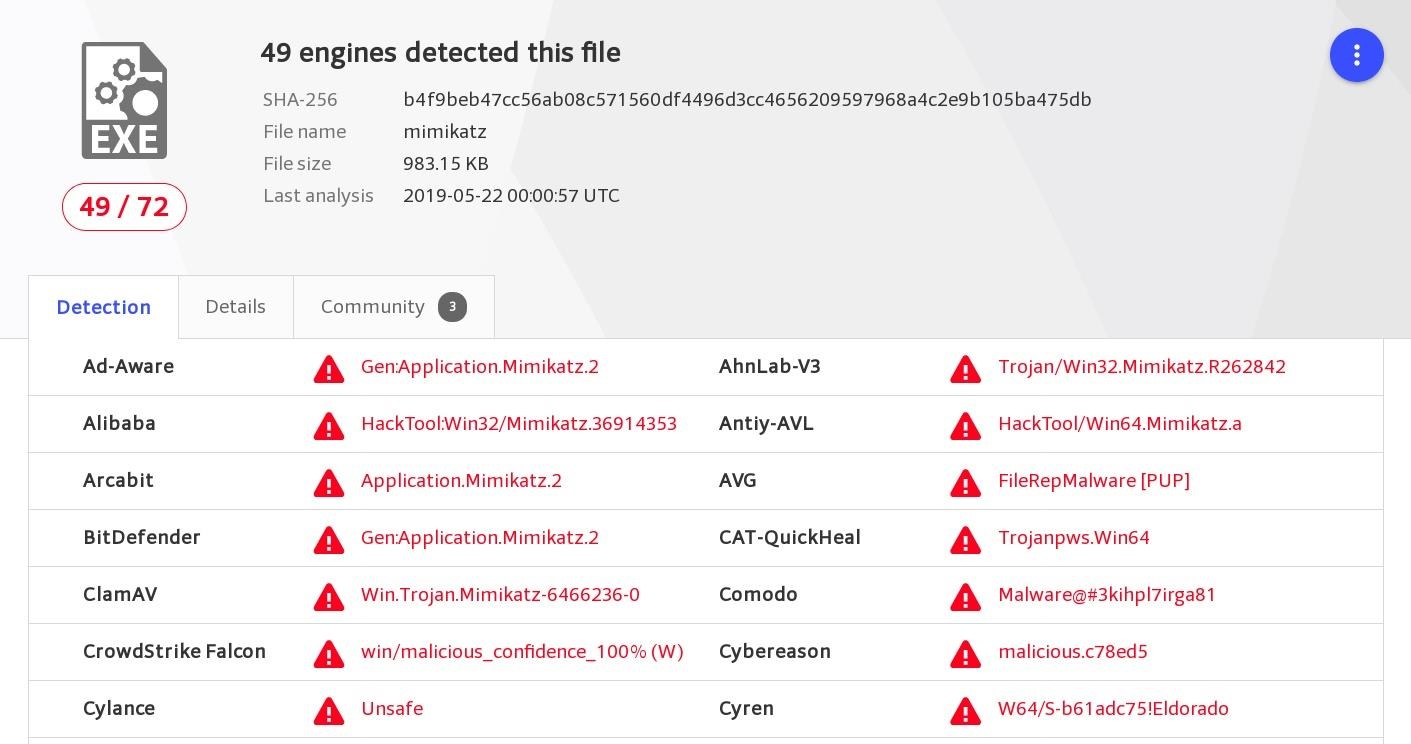
\includegraphics[width=120mm]{Immagini/2/mimikatz.jpg}
    \caption{MIMIKATZ e antivirus}
    \label{fig:MIMIKATZ}
\end{figure}

In combinazione con Mimikatz ora si utilizza ProcDump\cite{ProcDump}, un eseguibile autonomo progettato per gli amministratori per monitorare i crash dump delle applicazioni. ProcDump viene utilizzato per estrarre il dump LSASS \footnote[1]{\textbf{LSASS} : Local Security Authority Subsystem Service ( LSASS ) è un processo nei sistemi operativi Microsoft Windows che è responsabile dell'applicazione della politica di sicurezza sul sistema. Verifica gli utenti che accedono a un computer o server Windows, gestisce le modifiche alla password e crea token di accesso . Scrive anche nel registro di sicurezza di Windows .} , che viene successivamente spostato su un computer Windows offline e analizzato con Mimikatz . Questa è ancora una tecnica efficace per estrarre le credenziali da Windows, poiché ProcDump è un binario Microsoft firmato e non viene segnalato dalla maggior parte dei software antivirus.

\begin{figure}[h]
    \centering
    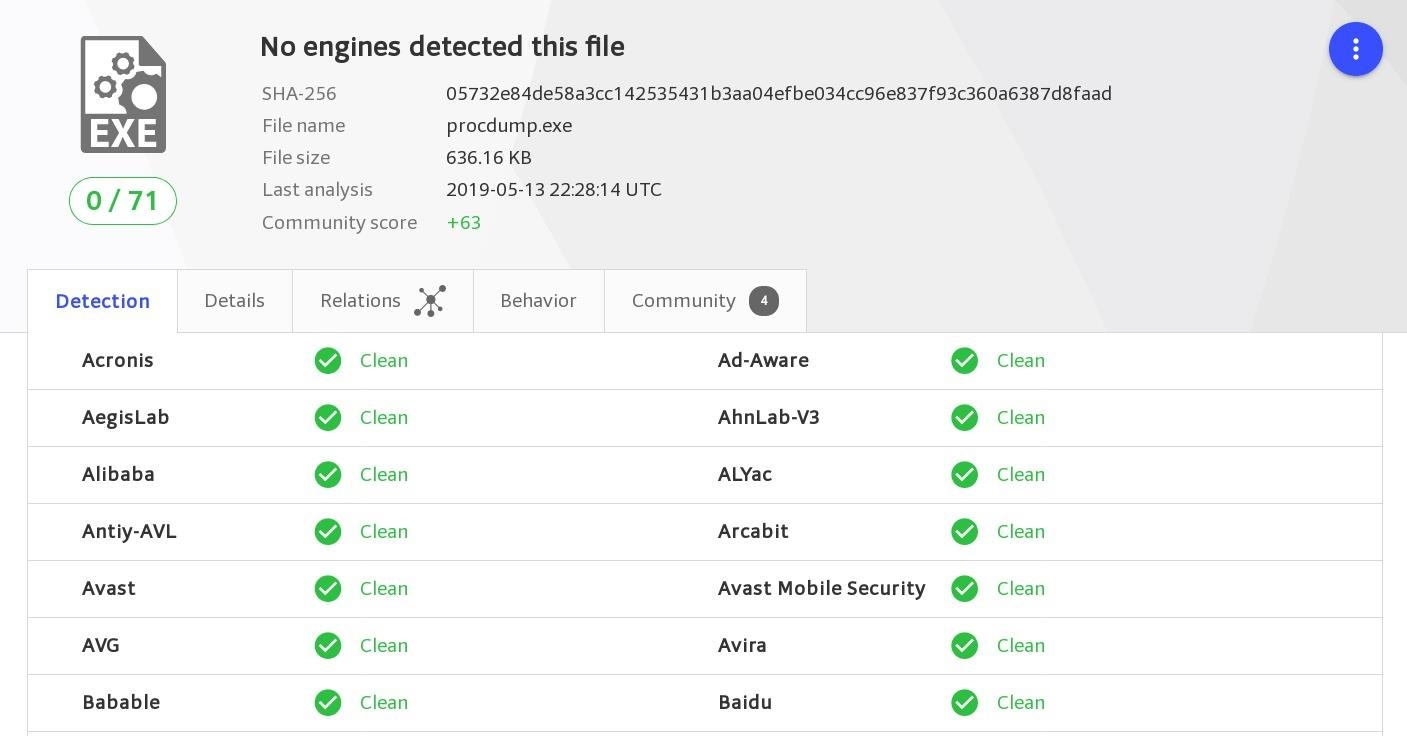
\includegraphics[width=120mm]{Immagini/2/procdump.jpg}
    \caption{ProcDump e antivirus}
    \label{fig:ProcDump}
\end{figure}

\section{Linux}
\section{MacOS}
\section{File}
\section{Network Hashes}
\section{Database hash extraction}
\section{Virtual Machines}
\subsection{VMware}
\subsection{Docker}
\subsection{Kubernetes}
\section{Cloud Services}
\subsection{AWS}
\subsection{GCP (Google Cloud Platform)}